\documentclass[a4paper, oneside]{article}
\usepackage{array}
\usepackage{shortvrb}
\usepackage{listings}
\usepackage{fullpage}
\usepackage{enumerate}
\usepackage{graphicx}
\usepackage{subfigure}
\usepackage{url}
\usepackage{indentfirst}
\usepackage{eurosym}
\usepackage{listings}
\usepackage{color}
\usepackage{fancybox}
\usepackage{ulem}
\usepackage{wrapfig}
\usepackage{systeme}
\usepackage{tabularx}
\usepackage{subfig}
\usepackage[dvipsnames]{xcolor}



\begin{document}
\begin{titlepage}
	\newcommand{\HRule}{\rule{\linewidth}{0.5mm}}
	\center
	\textsc{\LARGE Université de Liège}\\[1cm]
	\textsc{\Large Faculté des Sciences Appliquées}\\[2cm]
		
	\HRule \\[0.5cm]
	{ \huge \bfseries Automatic Multispeaker Voice Cloning Across Languages}\\[0.2cm]
	\HRule \\[3cm]

	\begin{minipage}{0.4\textwidth}
		\begin{flushleft} \Large
			\emph{Author:}\\
			Corentin \textsc{Jemine}
		\end{flushleft}
	\end{minipage}
	~
	\begin{minipage}{0.4\textwidth}
		\begin{flushright} \Large
			\emph{Supervisor:} \\
			Prof. Gilles \textsc{Louppe}
		\end{flushright}
	\end{minipage}\\[4cm]
	
	{\LARGE Academic year 2018 - 2019}\\[2cm]
	
	
\includegraphics{images/uliege_logo.jpg}\\[1.25cm]
	
	\textit{Graduation studies conducted for obtaining the Master's degree \\in Data Science by Corentin Jemine}
	
	\vfill
\end{titlepage}

\setcounter{page}{2}

\color{red}
Possibly, start with a TTS lexicon with some definitions. Meanwhile, I'll make a list of TSS-specific words that may be worth explaining: coarticulation, context, rich context, spectral envelope, fundamental frequency
\color{black}

\section{Abstract}
\color{red}
To do when I'll have a good overview of the project. Try to answer:
\begin{itemize}
	\item What is the goal of the application? What are its requirements, what is the setting, what kind of data are we going to use it on?
	\item What is zero-shot voice cloning? How does it fit in here (difference between an online and offline approach)?
	\item What are the particularities of our implementation (both model and datasets), what are its upsides and downsides (for example: requires huge datasets but fast inference)?
	\item What did we ultimately achieve? How good are our results?
\end{itemize}
\color{black}

\section{Introduction}

\color{red}
Concise presentation of the problem

GENERIC FRAMEWORK OF SPSS:

\color{black}
Statistical parametric speech synthesis (SPSS) refers to a group of TTS synthesis methods where the relation between features computed on the input text and output acoustic features are modeled by a statistical model (called an acoustic model). A complete SPSS framework thus also includes a pipeline to extract features from the text to synthesize as well as a system able to reconstruct an audio waveform from the acoustic features produced by the acoustic model (such a system is called a vocoder). Unlike the acoustic model, these two parts of the framework may be entirely engineered and make no use of statistical methods. If it is possible to condition the acoustic model in such a way that the characteristics of the generated voice are modified, then the framework is a multispeaker TTS synthesis system \color{red} could also be if conditioning on the vocoder. Rephrase this. \color{black}.

\color{red}
Processing of text into features (mainly linguistic contexts) - I haven't found a good source for this even though all the papers I cite use it... Maybe \cite{OnTheTrainingAspects} section 2.3 and 3.1.

SOTA ON MULTISPEAKER TTS:
\color{black}

Previous state of the art in SPSS includes hidden Markov models (HMM) based speech synthesis. In this framework, HMMs learn a distribution over mel-frequency cepstral coefficients (MFCC) with energy, their delta and delta-delta coefficients \cite{TTSSOTA}. These speech parameters are derived from the distributions output by HMMs using maximum likelihood  \color{red} talk about MLPG too. See "Speech parameter generation algorithms for HMMbased
speech synthesis" \color{black}. They are then fed through a vocoder, such as MLSA \cite{MLSA}. The input text to generate is processed into a sequence of linguistic contexts. The HMM parameters to use for speech generation are distributed conditionally to these contexts. Indeed, contexts are clustered with decision trees and an HMM is learned for each cluster \cite{HMMTTS}, effectively partitioning the training set. It is possible to modify the voice generated by conditioning on a speaker or tuning these parameters with adaptation or interpolation techniques (e.g. \cite{HMMSpeakerInterpolation}  \color{red} elaborate a bit on these techniques? \color{black}), making HMM-based speech synthesis a multispeaker TTS system. \color{red} Compare with concatenative see \cite{SPSSDNN} and https://ieeexplore.ieee.org/document/541110. Also, include the picture from \cite{Hashimoto-2015}? \color{black}

\begin{wrapfigure}{r}{7cm}
	\color{red} I'll take care of placing images correctly later... \color{black}
	\vspace{0cm}
	\centering
	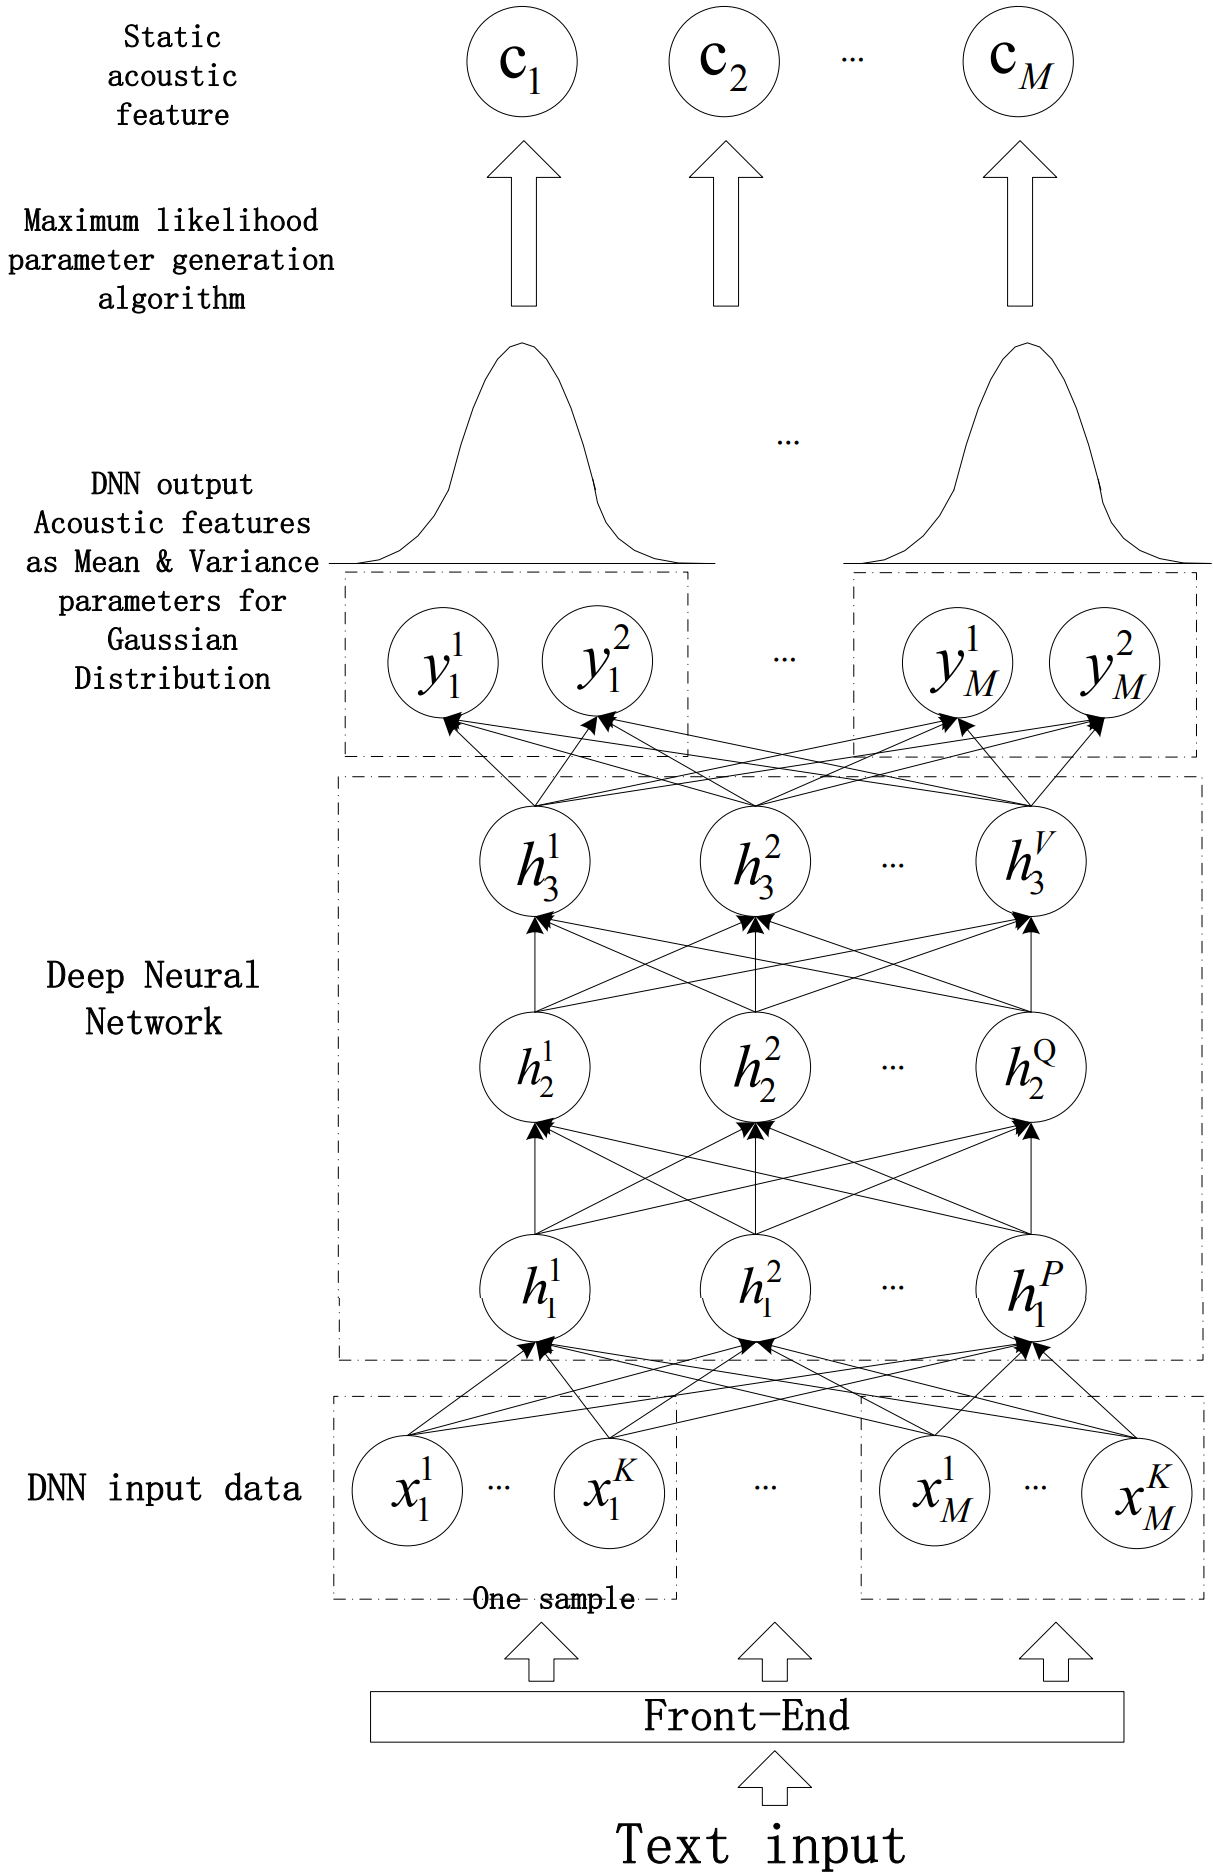
\includegraphics[width=7cm]{images/dnn_spss.png}
	\caption{General framework of the DNN-based TTS method \cite{Lu_combininga}}
	\label{dnn_tts_framework}
	\vspace{0cm}
\end{wrapfigure}

Improvements to this framework were later brought by feed-forward and recurrent deep neural networks (DNN and RNN respectively), as a result of progress in both hardware and software. \cite{SPSSDNN} proposes to replace entirely the decision tree-clustered HMMs in favor of a DNN. They argue for better data efficiency as the training set is no longer fragmented in different clusters of contexts\color{red}, and for a more powerful model?\color{black}. They demonstrate improvements over the speech quality with a number of parameters similar to that of the HMM-based approach. Later researches corroborate these findings \cite{OnTheTrainingAspects}.


\color{red}
Also read \cite{Yin2014ModelingDP}
\color{black}


\color{red}


Wavenet: breakthrough in TTS with raw waveform gen

Take images from https://deepmind.com/blog/wavenet-generative-model-raw-audio/ ?

Dilated causal convolutions

Condition on a speaker identity

Tacotron

Deep voice (1, 2, 3 + few samples), Tacotron 2

SV2TTS

Extensions?
\color{black}



\color{red}
\color{black}

\clearpage
\bibliographystyle{plain}
\bibliography{references} 




















%$$\Leftrightarrow h_b(x) =
%\left\{\begin{array}{lll}
%0 & if & P(y = 0 | x) > P(y = 1 | x)\\ 
%1 & else &
%\end{array}\right.$$



%\begin{figure}[h]
%	\centering
%	\includegraphics[width=16cm]{image.png}
%	\caption{caption}
%	\label{label}
%\end{figure}



%\begin{figure}[h]
%	\centering
%	\captionsetup{justification=centering}
%	\hspace{-1cm}
%	\subfigure{\includegraphics[height=5cm]{image.png}}
%	\subfigure{\includegraphics[height=5cm]{image.png}}
%	\hspace{-1cm}
%	\caption{caption}
%	\label{label}
%\end{figure}


%\begin{center}
%	\begin{tabular}{|r|ccc|ccc|}
%		\hline
%		& \multicolumn{6}{c|}{Validation set}\\
%		\hline
%		& \multicolumn{3}{c|}{Valid images (3126)} & \multicolumn{3}{c|}{Invalid images (3126)} \\
%		\hline
%		& Correct & Unclassified & Incorrect & Correct & Unclassified & Incorrect \\
%		\hline
%		Reduced & 94.98\% & 3.07\% & 1.95\% & 95.27\% & 2.91\% & 1.82\% \\
%		Lenet & 98.08\% & 0.74\% & 1.18\% & 97.86\% & 0.96\% & 1.18\% \\
%		\hline
%	\end{tabular}
%	
%	\vspace{0.5cm}
%	  
%	\begin{tabular}{|r|ccc|ccc|}
%		\hline
%		& \multicolumn{6}{c|}{Test set}\\
%		\hline
%		& \multicolumn{3}{c|}{Valid images (999)} & \multicolumn{3}{c|}{Invalid images (74)} \\
%		\hline
%		& Correct & Unclassified & Incorrect & Correct & Unclassified & Incorrect \\
%		\hline
%		Reduced& 94.29\% & 3.70\% & 2.00\% & 95.95\% & 4.05\% & 0.00\%  \\
%		Lenet & 96.90\% & 1.30\% & 1.80\% & 97.30\% & 1.35\% & 1.35\% \\
%		\hline
%	\end{tabular}
%\end{center}


\end{document}













































































































